%%% Copyright (C) 2018 Vincent Goulet
%%%
%%% Ce fichier fait partie du projet
%%% «Programmer avec R»
%%% https://gitlab.com/vigou3/programmer-avec-r
%%%
%%% Cette création est mise à disposition selon le contrat
%%% Attribution-Partage dans les mêmes conditions 4.0
%%% International de Creative Commons.
%%% https://creativecommons.org/licenses/by-sa/4.0/

%%%
%%% Page de titre
%%%

%% Normes de présentation visuelle 2018
%%
%% - grille de 8 unités de haut
%% - 1 mesure = 1/8 d'unité
%% - bande identitaire de 1 mesure placée au bas de la 7e unité
%% - logo haut de 4 mesures avec blancs de deux mesures en haut et
%%   en bas
%% - blanc équivalent à la largeur du blason à droite du logo
%% - bande or de la largeur du logo + blanc à droite
%%
%% Dimensions du logo UL
%%
%% hauteur: 128
%% largeur totale: 310
%% largeur blason: 100
%% valeur clé: (310 + 100)/128 = 3.2031125
%%
%% Dimension de l'image
%%
%% hauteur: 55 mesures - 1pt (filet) = 54.9191919 mesures
%% largeur: 8.5in
%% ratio largeur/hauteur: 8.5/9.4392

\begingroup
\TPGrid{8.5}{64}
\textblockorigin{0mm}{0mm}
\setlength{\parindent}{0mm}
\setlength{\imageheight}{54.9191919\TPVertModule}
\setlength{\logoheight}{4\TPVertModule}
\setlength{\bandeorwidth}{3.203125\logoheight}
\setlength{\banderougewidth}{\paperwidth}
\addtolength{\banderougewidth}{-\bandeorwidth}
\setlength{\bandeorheight}{\TPVertModule}
\setlength{\banderougeheight}{\TPVertModule}
\setlength{\textwidth}{\paperwidth}
\addtolength{\textwidth}{-2\TPHorizModule}

\def\titlefmt{%
  \sffamily\bfseries\fontsize{52}{52}\selectfont\thetitle}
\def\authorfmt{%
  \sffamily\mdseries\fontsize{28}{38}\selectfont\theauthor}
\def\affiliation{%
  \sffamily\mdseries\fontsize{16}{20}\selectfont
  Professeur titulaire \\
  École d'actuariat, Université Laval}
\def\edition{%
  \sffamily\mdseries\fontsize{16}{16}\selectfont
  Édition {\fullcaps\year}.\month}

%% bandeau identitaire
\begin{textblock*}{\paperwidth}[0,1](0mm,56\TPVertModule)
  \textcolor{rouge}{\rule{\banderougewidth}{\banderougeheight}}% % bande rouge
  \textcolor{or}{\rule{\bandeorwidth}{\bandeorheight}}           % bande or
\end{textblock*}

%% logo UL
\begin{textblock*}{\bandeorwidth}(\banderougewidth,58\TPVertModule)
  
\includegraphics[height=\logoheight,%
                   keepaspectratio=true]{images/ul_p}
\end{textblock*}

%% image de fond
\begin{textblock*}{\paperwidth}(0mm,0mm)
  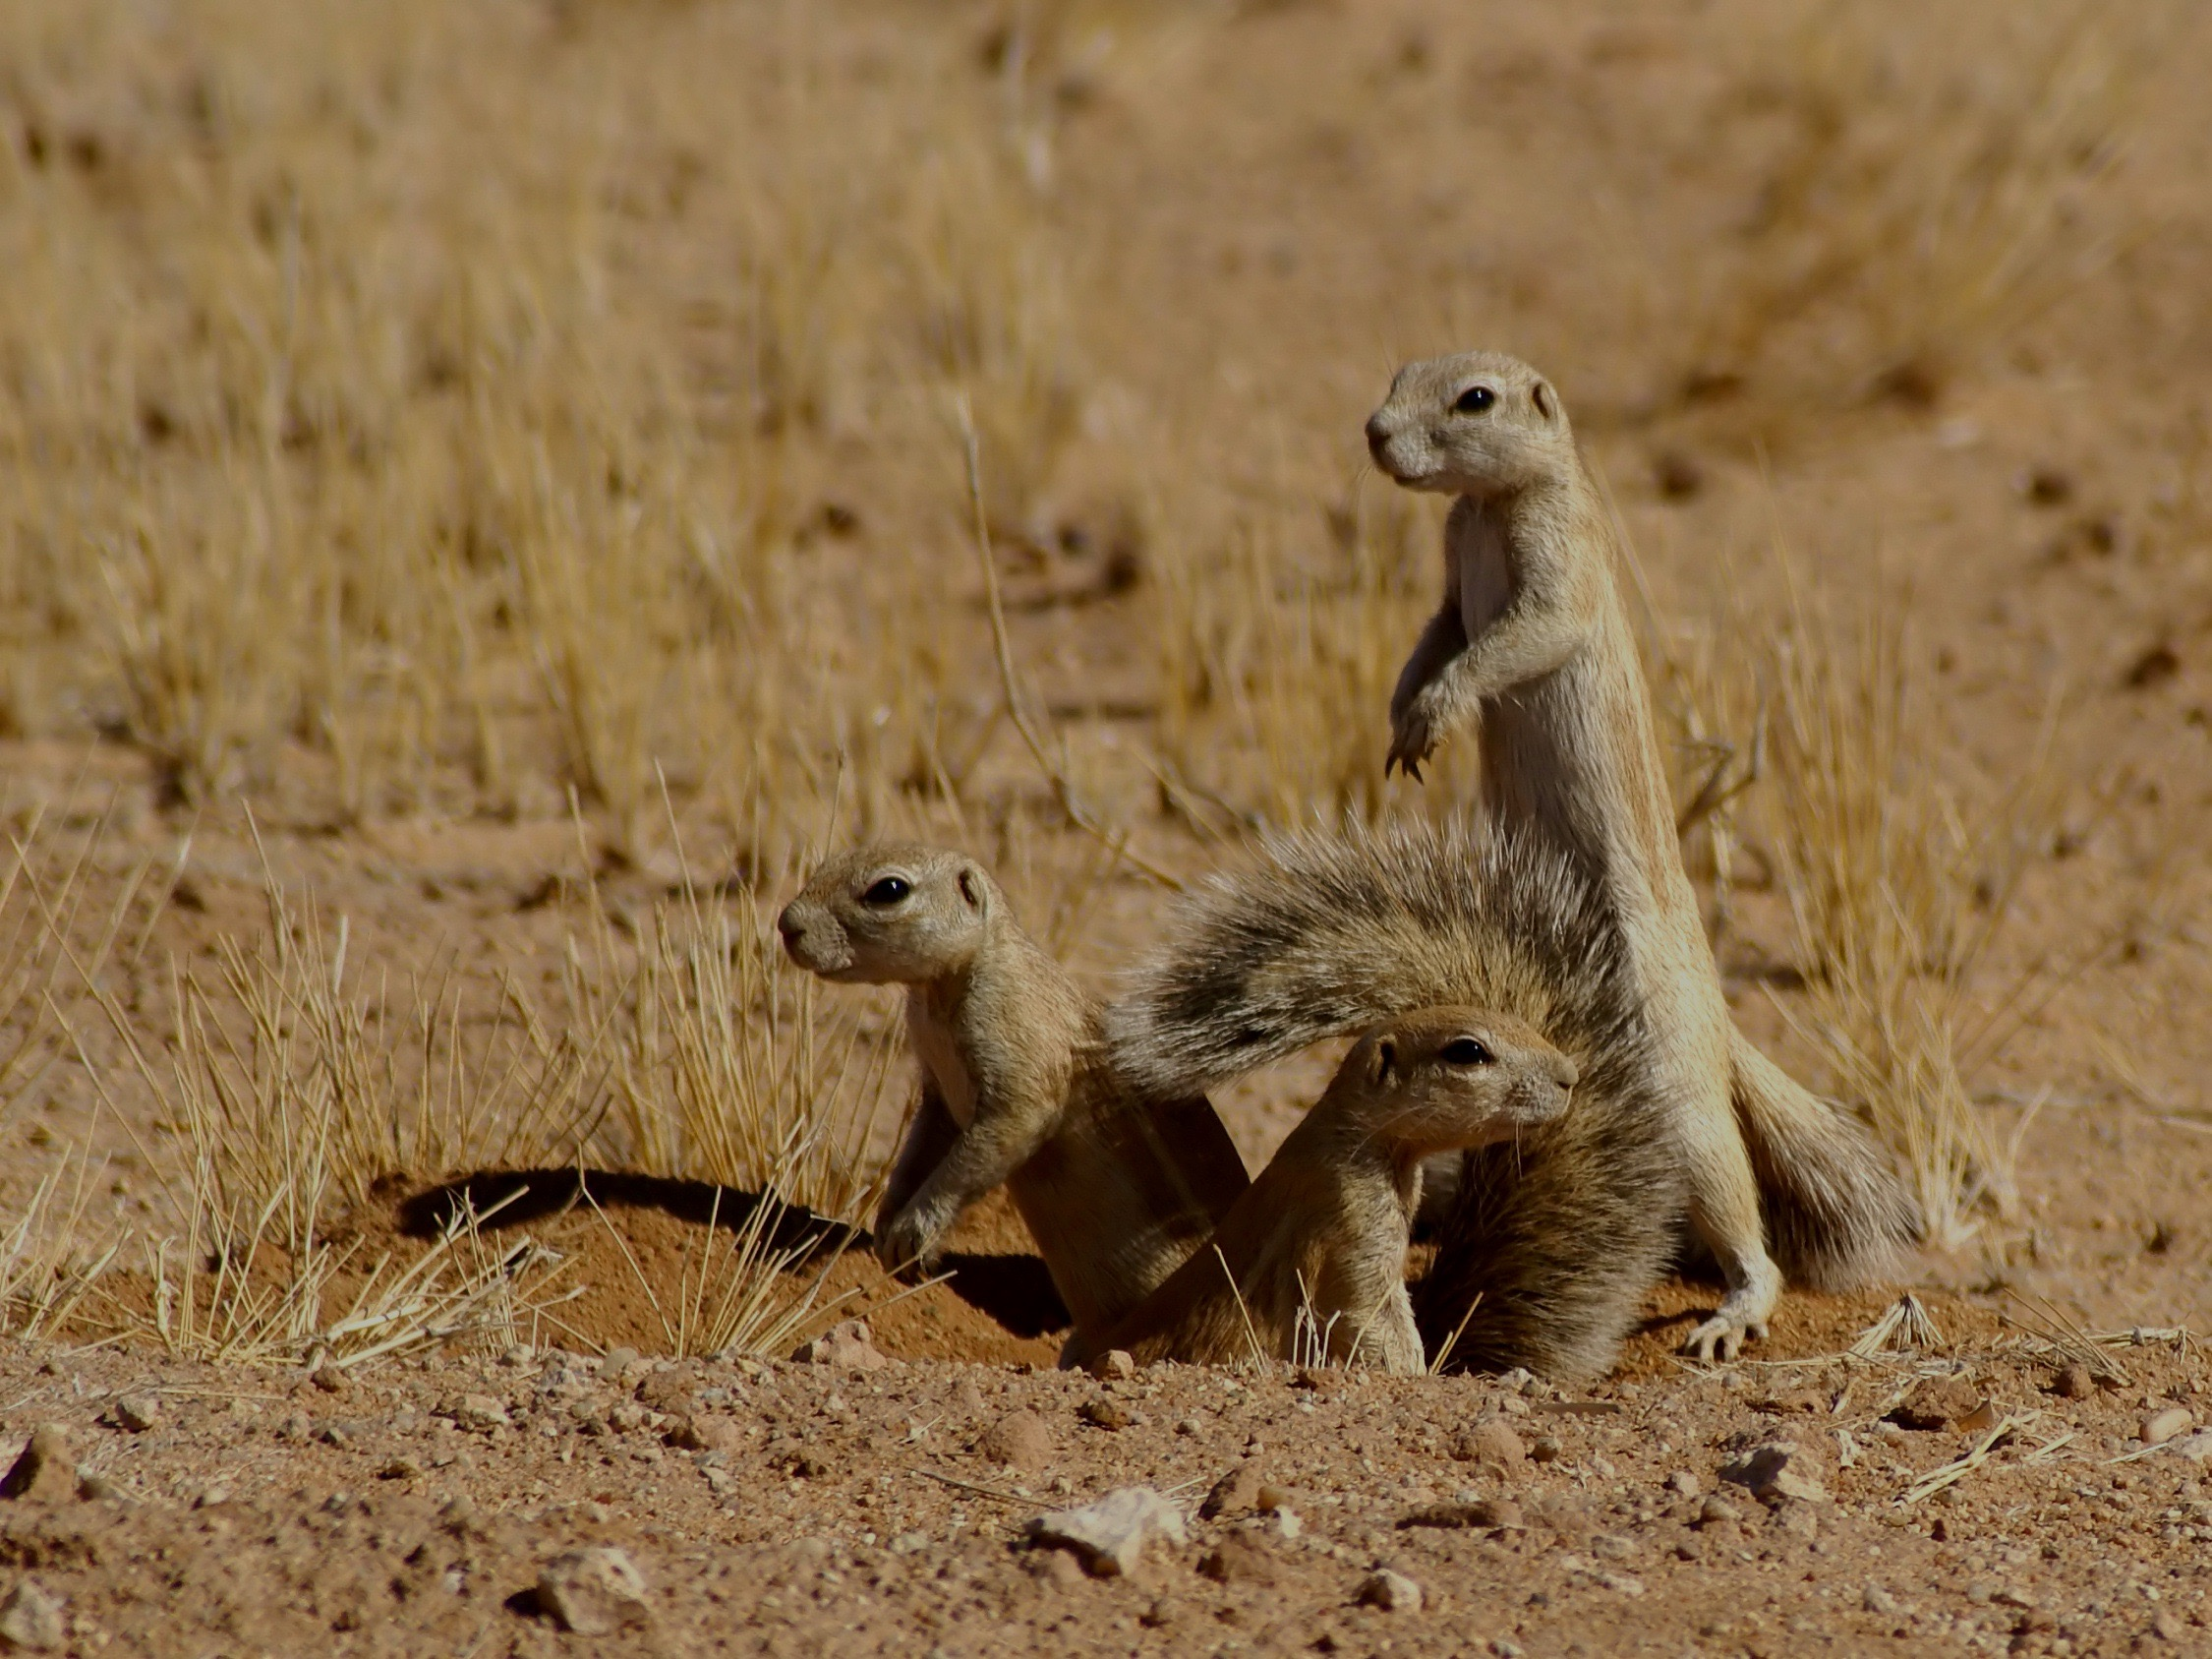
\includegraphics[height=\imageheight,%
                   width=\paperwidth,%
                   trim=535 0 196 0,clip]{images/Xerus_inauris_1}
\end{textblock*}

%% titre
\begin{textblock*}{\textwidth}(\TPHorizModule,6\TPVertModule)
  \textcolor{black!10}{\titlefmt}
\end{textblock*}

%% auteur
\begin{textblock*}{\textwidth}(\TPHorizModule,11.5\TPVertModule)
  \textcolor{black!10}{\authorfmt}
\end{textblock*}

\null\cleardoublepage

%%%
%%% Page frontispice
%%%

%% titre
\begin{textblock*}{\textwidth}(\TPHorizModule,6\TPVertModule)
  \titlefmt
\end{textblock*}

%% auteur
\begin{textblock*}{\textwidth}(\TPHorizModule,11.5\TPVertModule)
  \authorfmt
\end{textblock*}

%% affiliation
\begin{textblock*}{\textwidth}(\TPHorizModule,15.5\TPVertModule)
  \affiliation
\end{textblock*}

%% édition
\begin{textblock*}{\textwidth}(\TPHorizModule,58\TPVertModule)
  \edition
\end{textblock*}
\endgroup

%%% Local Variables:
%%% mode: latex
%%% TeX-master: "programmer-avec-r"
%%% TeX-engine: xetex
%%% End:
